\documentclass[12pt]{article}
\usepackage[a4paper, left=5mm, right=5mm, top=5mm, bottom=5mm]{geometry}
%\usepackage[a4paper, top=15mm, right=10mm, bottom=10mm, left=10mm]{geometry}
\usepackage[russian]{babel}
\usepackage{fontspec}
\usepackage{graphicx}
\usepackage[unicode]{hyperref}
\usepackage{enumitem}
\usepackage{wrapfig}
\usepackage{tabularx}
\usepackage{amssymb}
\usepackage{gensymb}
\usepackage{amsmath}
\usepackage{blindtext}
\usepackage{float}
\usepackage{multicol}
\usepackage{latexsym}
%\usepackage[font={bf}, name={Рис. }, justification=justified]{caption}
\usepackage{caption}
\usepackage{subcaption}
\usepackage{listings}
\usepackage{xcolor}
\usepackage{breqn}
\usepackage{pdfpages}

\setmainfont{Times New Roman}
\righthyphenmin=2 % правильные переносы
%\graphicspath{{images/}} % путь к картинкам

% Стиль кода для 5 задания
\lstdefinestyle{mystyle}{
	backgroundcolor=\color{backcolour},   
	commentstyle=\color{codegreen},
	keywordstyle=\color{magenta},
	numberstyle=\tiny\color{codegray},
	stringstyle=\color{codepurple},
	basicstyle=\ttfamily\footnotesize,
	breakatwhitespace=false,         
	breaklines=true,                 
	captionpos=b,                    
	keepspaces=true,                 
	numbers=none,                    
	numbersep=5pt,                  
	showspaces=false,                
	showstringspaces=false,
	showtabs=false,                  
	tabsize=2
}
\lstset{style=mystyle}

\title{Lab6 OPD}
\author{Азат Сиразетдинов}

\begin{document}
	\thispagestyle{empty}
	\begin{center}
		Федеральное государственное автономное образовательное учреждение\\ 
		высшего образования\\
		«Национальный исследовательский университет ИТМО»\\
		\textit{Факультет Программной Инженерии и Компьютерной Техники}\\
	\end{center}
	\vspace{2cm}
	\begin{center}
		\large
		\textbf{Лабораторная работа № 6}\\
		по дисциплине ОПД\\
		Обмен по прерыванию\\
		Вариант № 1323
	\end{center}
	\vspace{7cm}
	\begin{flushright}
		Выполнил:\\
		cтудент  группы P3116\\
		Сиразетдинов А. Н\\
		Преподаватель: \\
		Афанасьев Д. Б.\\
	\end{flushright}
	\vspace{6cm}
	\begin{center}
		г. Санкт-Петербург\\
		2023г.
	\end{center}
	\newpage
	
	\tableofcontents
	
	\newpage
	\section{Задание}
	
	По выданному преподавателем варианту разработать и исследовать работу комплекса программ обмена данными в режиме прерывания программы. Основная программа должна изменять содержимое заданной ячейки памяти (Х), которое должно быть представлено как знаковое число. Область допустимых значений изменения Х должна быть ограничена заданной функцией F(X) и конструктивными особенностями регистра данных ВУ (8-ми битное знаковое представление). Программа обработки прерывания должна выводить на ВУ модифицированное значение Х в соответствии с вариантом задания, а также игнорировать все необрабатываемые прерывания.
	\begin{itemize}
		\item Основная программа должна уменьшать на 3 содержимое X (ячейки памяти с адресом 03916) в цикле.
		\item Обработчик прерывания должен по нажатию кнопки готовности ВУ-3 осуществлять вывод результата вычисления функции F(X)=3X+6 на данное ВУ, a по нажатию кнопки готовности ВУ-2 изменить знак содержимого РД данного ВУ и записать в Х
		\item Если Х оказывается вне ОДЗ при выполнении любой операции по его изменению, то необходимо в Х записать максимальное по ОДЗ число.
	\end{itemize}
	\newpage
	
	\section{Описание программы}
	\subsection{Назначение программы}
	Программа изменяет значение ячейки $ 039 $
	
	\subsection{Область представления}
	X - знаковое целое 16-разрядное число, значащими являются 8 младших разрядов
	
	\subsection{Область допустимых значений}
	
	$ X \in \left[-2C;28\right] $
	
	\subsection{Расположение программы и данных}
	Программа располагается в ячейках с 50 по 65
	Вектора прерываний располагаются в ячейках с 0 по F
	Обработчики прерываний располагаются в ячейках с 10 по 22
	Исходные данные располагаются в ячейках:
	\begin{itemize}
		\item 39 - Х
	\end{itemize}
	Константы данные располагаются в ячейках:
	\begin{itemize}
		\item 40 - Х_MAX со значением 28
		\item 41 - Х_MIN со значением -2C
	\end{itemize}
	
	\section{Исходный код программы}
	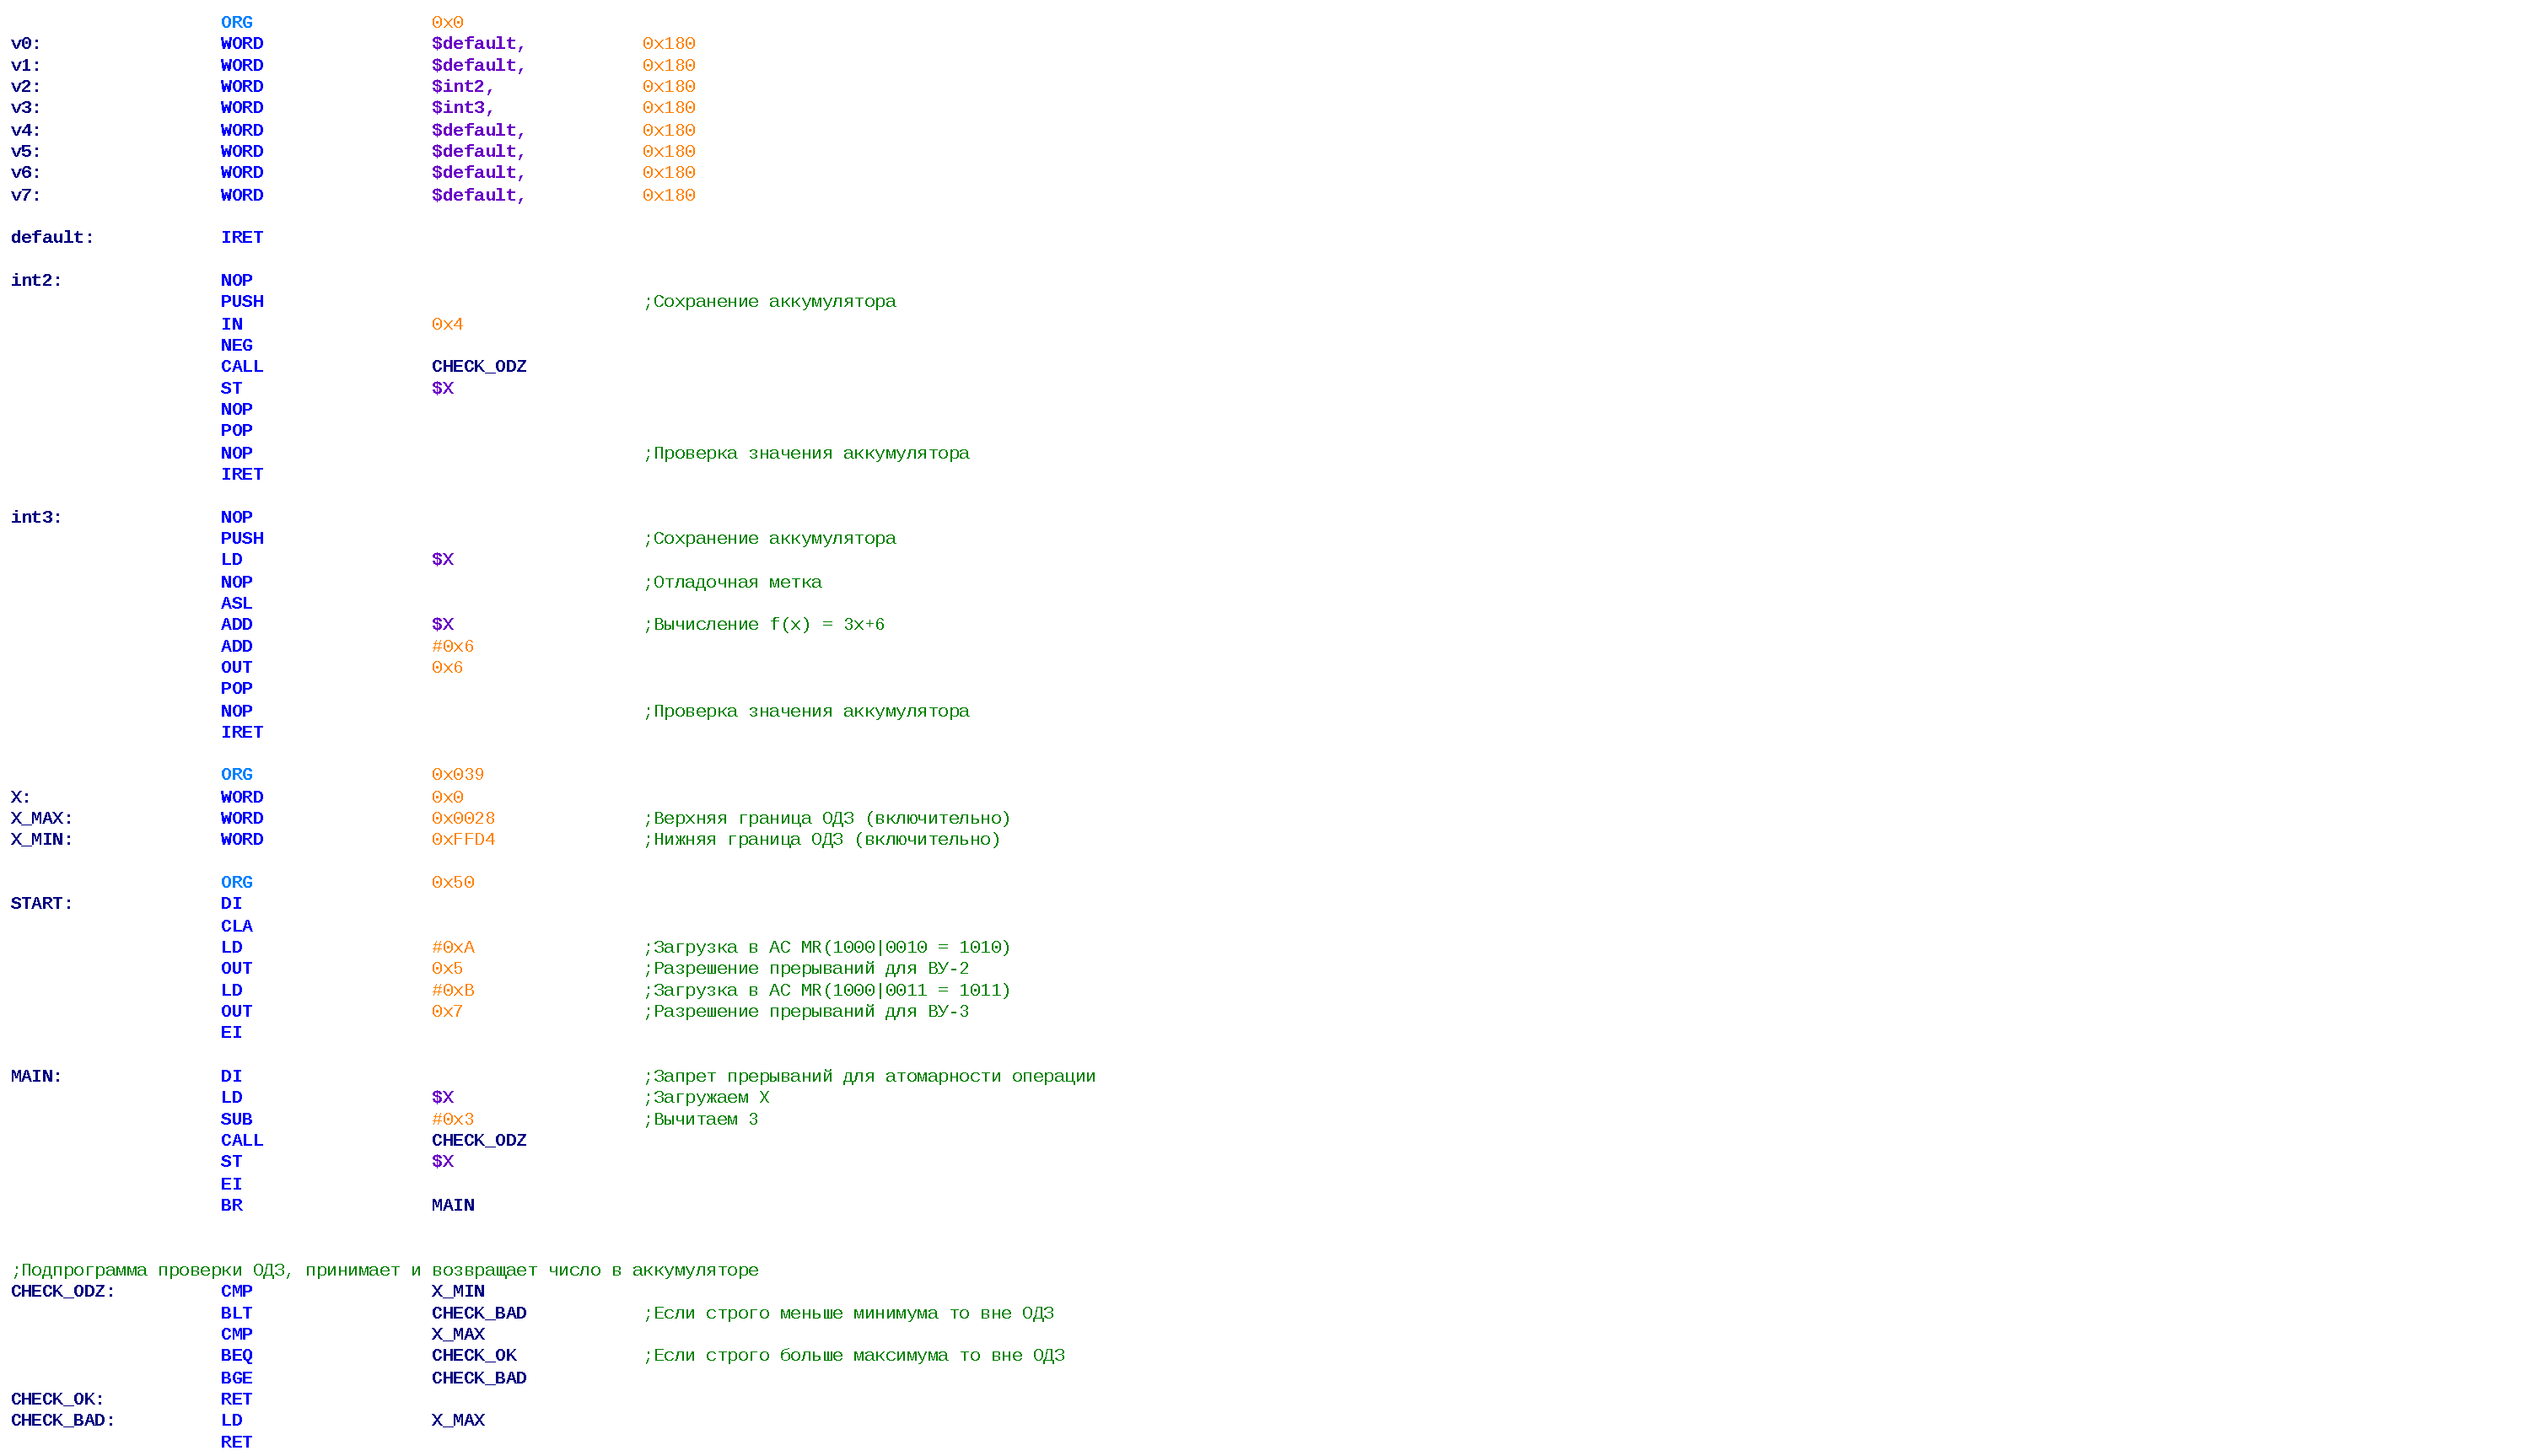
\includegraphics[width=0.9\linewidth]{colored_code.pdf}
	\newpage
	
	\section{Методика проверки}
	\begin{enumerate}[]
		\item Загрузить комплекс программ в память базовой ЭВМ
		\item Изменить значение точки останова по адресу 18 на HLT
		\item Изменить значение точки останова по адресу 1D на HLT
		\item Запустить программу в автоматическом режиме с адреса 50
		\item Открыть "КВУ-2"
		\item Установить значение 1000000 (вне ОДЗ)
		\item Установить "Готовность КВУ-2"
		\item Дождаться останова
		\item Проверить что значение AC равно 01010011 (X_MAX)
		\item Продолжить исполнение программы
		\item Открыть "КВУ-2"
		\item Установить значение 00101100
		\item Установить "Готовность КВУ-2"
		\item Дождаться останова
		\item Проверить что значение AC равно 00101100
		\item Продолжить исполнение программы
		\item Открыть "КВУ-3"
		\item Установить "Готовность КВУ-3"
		\item Дождаться останова
		\item Записать значение AC как переменную х
		\item Продолжить исполнение программы
		\item Дождаться погасания кнопки "Готовность КВУ-3"
		\item Сопоставить значение DR ВУ-3 и ожидаемым значением формулы 3x+6
	 \end{enumerate}
 	\newpage
 
 	\section{Вывод}
 	В процессе выполнения лабораторной работы я узнал про работу с внешними устройствами по прерыванию и про блокировку для предоставление атомарности операции. Была написана программа реализующую работу с прерываниями ВУ-2 и ВУ-3 и разработана методика проверки. 
\end{document}







